\subsection{From Intuition to Inertia: Euler Formalizes Galileo's Hunches}

Euler didn’t stop at fixing notation. He looked at physics—the way objects move, spin, and resist motion—and asked the question that made him the legend we know today:

\begin{quote}
\textbf{“What if we actually did the math?”}
\end{quote}

One of the places where this mindset really shined was in the study of \textbf{rotation}—specifically, the concept of \textbf{moment of inertia}.


\begin{figure}[H]
\centering
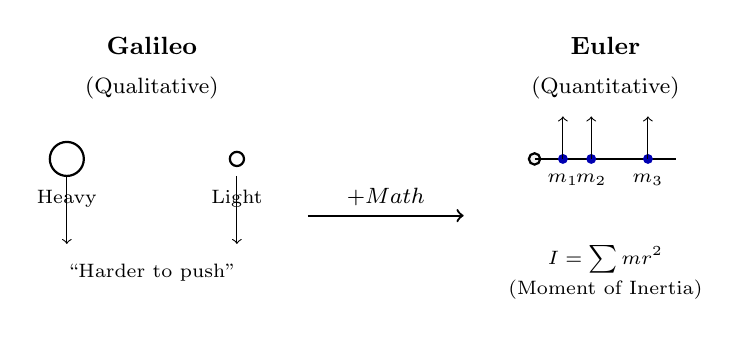
\begin{tikzpicture}[scale=1.8, every node/.style={font=\small}]

  % Left side: Galileo's intuition
  \node[align=center] at (0,2.8) {\textbf{Galileo}};
  \node at (0,2.5) {\footnotesize (Qualitative)};
  \draw[thick] (-0.6,2.0) circle (0.12);
  \draw[thick] (0.6,2.0) circle (0.05);
  \node[below] at (-0.6,1.85) {\scriptsize Heavy};
  \node[below] at (0.6,1.85) {\scriptsize Light};
  \draw[->] (-0.6,1.88) -- (-0.6,1.4);
  \draw[->] (0.6,1.88) -- (0.6,1.4);
  \node at (0,1.2) {\scriptsize “Harder to push”};

  % Arrow from intuition to math
  \draw[->, thick] (1.1,1.6) -- (2.2,1.6);
  \node[above] at (1.65,1.6) {\footnotesize $\text{+ Math}$};

  % Right side: Euler’s formalism
  \node[align=center] at (3.2,2.8) {\textbf{Euler}};
  \node at (3.2,2.5) {\footnotesize (Quantitative)};
  \draw[thick, fill=gray!10] (2.7,2.0) circle (0.04);
  \draw[thick] (2.7,2.0) -- (3.7,2.0);

  % Masses along the rod
  \foreach \x/\label in {2.9/m_1, 3.1/m_2, 3.5/m_3} {
    \fill[blue!70!black] (\x,2.0) circle (0.035);
    \node[below=2pt] at (\x,2.0) {\scriptsize $\label$};
    \draw[->, thin] (\x,2.0) -- (\x,2.3);
  }

  % Label for I = sum m r^2
  \node[align=center] at (3.2,1.2) {
    \scriptsize $I = \sum m r^2$ \\
    \scriptsize (Moment of Inertia)
  };

\end{tikzpicture}
\caption{Galileo knew heavier objects were harder to move. Euler turned that intuition into math — introducing the moment of inertia $I = \sum m r^2$, quantifying rotational resistance.}
\end{figure}



\subsubsection{Galileo’s Gut Feeling}

Before Euler came along with his calculus war cleanup crew, Galileo had already been exploring how objects move. He had a brilliant physical intuition and could describe how bodies accelerated, rolled, or fell. 

But Galileo's take on rotational motion was still pretty fuzzy. He understood that spinning objects seemed to resist changes in their spin, and that mass and distance from the axis mattered somehow—but his explanations were mostly qualitative. He talked about "heaviness of rotation" without formalizing what that actually meant.

He knew something was happening, but he couldn’t quite bottle it up in an equation.


\begin{figure}[H]
\centering
\begin{tikzpicture}[scale=2.5, every node/.style={font=\small}]

  % Wheel (circle)
  \draw[thick] (0,0) circle (1);

  % Central axis
  \fill[black] (0,0) circle (0.03);
  \node[below right=2pt] at (0,0) {Axis};

  % Mass points around the edge
  \foreach \angle in {0, 90, 180, 270} {
    \coordinate (P) at ({cos(\angle)}, {sin(\angle)});
    \fill[blue] (P) circle (0.05);
    \node at ($(P)+(0.2,0.1)$) {\scriptsize Mass};
  }

  % Arrows indicating rotation
  \draw[->, thick, red!60!black] (1.1,0) arc[start angle=0, end angle=90, radius=1.1];
  \node[red!60!black] at (0.8,0.7) {\scriptsize Spinning};

  % Question mark to indicate qualitative feel
  \node at (-1.1,-0.8) {\Large \textbf{?}};
  \node[align=center] at (0,-1.2) {
    \scriptsize ``Heaviness of rotation'' \\
    \scriptsize (Galileo's intuition)
  };

\end{tikzpicture}
\caption{Galileo sensed that mass and distance from the axis affected rotation, but lacked the tools to formalize it. His intuition hinted at what Euler would later define as moment of inertia.}
\end{figure}



\subsubsection{Euler’s Turn: Defining Rotational Resistance}

Euler stepped in and gave that "heaviness of rotation" a name—and more importantly, a formula.

\[
I = \sum m r^2
\]

Where:
\begin{itemize}
    \item \( I \) is the \textbf{moment of inertia}
    \item \( m \) is the mass of a point in the object
    \item \( r \) is the distance from that point to the axis of rotation
\end{itemize}

In other words: the farther mass is from the center, the more it resists rotational acceleration. And unlike Galileo, Euler didn’t just say this. He proved it. With math. 

He generalized it, extended it to rigid bodies, and tied it directly into his \textbf{Euler’s Laws of Motion}—a rotational analog to Newton’s laws. It wasn’t just about mass anymore; it was about how that mass was distributed. This was the foundation of \textbf{rotational dynamics} as we know it today.


\begin{figure}[H]
\centering
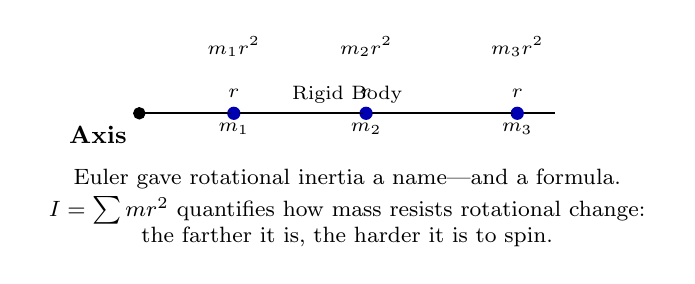
\begin{tikzpicture}[scale=2.4, every node/.style={font=\small}]

  % Axis of rotation
  \filldraw[black] (0,0) circle (0.03);
  \node[below left=1pt] at (0,0) {\textbf{Axis}};

  % Rod or body
  \draw[thick] (0,0) -- (2.2,0);
  \node[above] at (1.1,0) {\scriptsize Rigid Body};

  % Point masses and radius vectors
  \foreach \x/\mass in {0.5/m_1, 1.2/m_2, 2.0/m_3} {
    \fill[blue!70!black] (\x,0) circle (0.035);
    \draw[dashed] (0,0) -- (\x,0);
    \node[below] at (\x,0) {\scriptsize $\mass$};
    \node[above] at (\x,0.03) {\scriptsize $r$};
    \node[above=10pt] at (\x,0.1) {\scriptsize $\mass r^2$};
  }

  % Moment of inertia label
  \node at (1.1,-0.5) {
    \begin{minipage}{0.65\linewidth}
      \centering
      \footnotesize Euler gave rotational inertia a name—and a formula. \\
      \vspace{2pt}
      $I = \sum m r^2$ quantifies how mass resists rotational change: the farther it is, the harder it is to spin.
    \end{minipage}
  };

\end{tikzpicture}
\caption{Euler defined rotational resistance with the moment of inertia: $I = \sum m r^2$. It’s not just mass—it’s where that mass is placed.}
\end{figure}



\subsubsection{The Controversy: Who Really Deserved the Credit?}

Now, as with all great ideas in science, credit is complicated.

Some argue that Euler didn’t “discover” the moment of inertia so much as refine what Galileo and others had already hinted at. After all, rotational resistance had been observed and described centuries earlier.

But here’s the thing: \textbf{Euler named it}, derived the equations, applied it across multiple physical systems, and baked it directly into his larger mechanical framework. He took a vague physical intuition and turned it into a quantifiable, generalizable tool.

That’s the difference between noticing that spinning things are hard to stop—and building the math that can model a satellite, a spinning top, or a collapsing star.

\subsubsection{The Real Power Move: Abstracting Physics into Calculus}

Euler didn’t just do math. He rewrote physics using math.

He wasn’t content to say “this thing spins weird.” He asked: “How can I describe spinning with the same language I use to describe straight-line motion?”

And he succeeded.

Thanks to Euler:
\begin{itemize}
    \item We can model rotational kinetic energy: \( \frac{1}{2} I \omega^2 \)
    \item We have Euler’s equations of motion for rigid bodies
    \item We can launch spacecraft, design gyroscopes, and simulate 3D physics in video games
\end{itemize}

Galileo laid the philosophical groundwork. Euler built the infrastructure.

\begin{center}
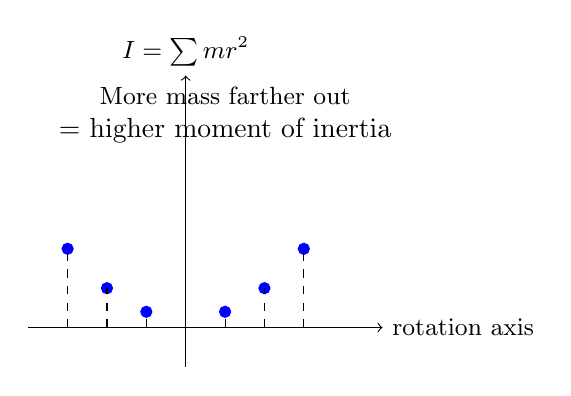
\begin{tikzpicture}[scale=1.0]
    % Axis
    \draw[->] (-2,0) -- (2.5,0) node[right] {\small rotation axis};
    \draw[->] (0,-0.5) -- (0,3.2) node[above] {\small $I = \sum m r^2$};

    % Mass points and distances
    \foreach \x in {-1.5,-1,-0.5,0.5,1,1.5} {
        \filldraw[blue] (\x, {0.1 + 0.4*\x*\x}) circle (2pt);
        \draw[dashed] (\x,0) -- (\x, {0.1 + 0.4*\x*\x});
    }

    \node[align=center] at (0.5, 2.7) {\small More mass farther out \\ = higher moment of inertia};
\end{tikzpicture}
\end{center}

So next time you see something spinning and refusing to stop, thank Galileo for noticing—and Euler for explaining.
